\begin{answer}

HOW TO OBSERVATIONS IN THE PLOT?

CODE TEMPLATE: 1) NEED TO EDIT OUT SIDE OF ***START HERE*** NO NEED TO LOAD FOR EACH LOOP 2) NEED K=1 AND K=2? 3) OVERWRITTING K=[] OK?

With k increasing, the fitting is getting better. So it requires a relatively high degree k to fit the given training data
\begin{figure}
    \centering
    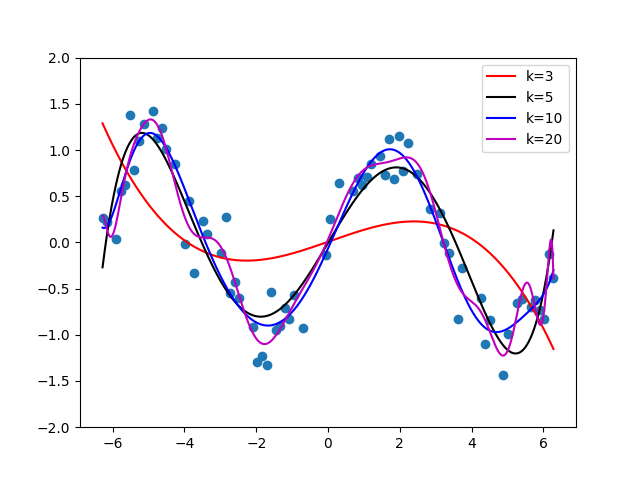
\includegraphics[width=0.5\linewidth]{ps1_q3_(c).png}
    \caption{ps1\_q3\_(c)}
    \label{fig:enter-label}
\end{figure}
\end{answer}
